\documentclass[border=10]{standalone}
\usepackage{tikz}

% Directory Tree settings 
\makeatletter
\newcount\dirtree@lvl
\newcount\dirtree@plvl
\newcount\dirtree@clvl
\def\dirtree@growth{%
  \ifnum\tikznumberofcurrentchild=1\relax
  \global\advance\dirtree@plvl by 1
  \expandafter\xdef\csname dirtree@p@\the\dirtree@plvl\endcsname{\the\dirtree@lvl}
  \fi
  \global\advance\dirtree@lvl by 1\relax
  \dirtree@clvl=\dirtree@lvl
  \advance\dirtree@clvl by -\csname dirtree@p@\the\dirtree@plvl\endcsname
  \pgf@xa=0.5cm\relax % horizontal margin
  \pgf@ya=-0.75cm\relax % vertical margin
  \pgf@ya=\dirtree@clvl\pgf@ya
  \pgftransformshift{\pgfqpoint{\the\pgf@xa}{\the\pgf@ya}}%
  \ifnum\tikznumberofcurrentchild=\tikznumberofchildren
  \global\advance\dirtree@plvl by -1
  \fi
}

\tikzset{
  dirtree/.style={
    growth function=\dirtree@growth,
    every node/.style={anchor=north},
    every child node/.style={anchor=west},
    edge from parent path={(\tikzparentnode\tikzparentanchor) |- (\tikzchildnode\tikzchildanchor)}
  }
}

\makeatother

\begin{document}

	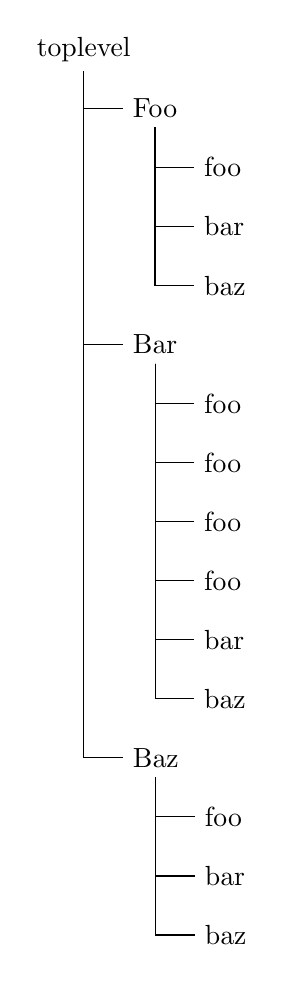
\begin{tikzpicture}[dirtree]
	\node {toplevel} 
	    child { node {Foo}
	            child { node {foo} }
	            child { node {bar} }
	            child { node {baz} }
	    }
	    child { node {Bar}
	        child { node {foo} }
	        child { node {foo} }
	        child { node {foo} }
	        child { node {foo} }
	        child { node {bar} }
	        child { node {baz} }
	    }
	    child { node {Baz}
	        child { node {foo} }
	        child { node {bar} }
	        child { node {baz} }
	    };
	\end{tikzpicture}

\end{document}